
\chapter{Konfidenční množiny, Intervaly spolehlivosti}
Bodové odhady $\widehat{\t}_n(\X)=\widehat{\t}_n$, resp. $T_n(\X)=T_n$, sice poskytují odhad hodnoty daného parametru, nicméně například ve~spojitém statistickém modelu (ASR$_\lambda$) vždy platí, že\\ $\PP\br{\htn(\X)=\t_0}=0,~\forall\t_0$, resp. $\PP\br{T_n(\X)=\tau(\t)}=0,~\forall\t\in\Theta$. Z~tohoto důvodu se~zavádí tzv. interval spolehlivosti, což je interval, ve~kterém se~neznámý parametr $\t$ nachází s~námi zadanou pravděpodobností (například 95\%). Přesnost takového odhadu je pak dán šířkou tohoto intervalu.


\begin{define}
	Nechť $\X=(X_1,...,X_n)\sim\PP\in\mathscr{P}$ na~$(\Omega,\mathcal{A})$, označme $\theta=\theta(\PP)\in\Theta\subset\R^1$ funkcionál na~$\mathscr{P}$, resp. $\theta\in\Theta\subset\R^k$. Označíme $\Bb_\Theta$ systém borelovských podmnožin $\Theta$ a~zvolíme číslo $\alpha\in(0,1)$. Pak $C(\X)\in\Bb_\Theta$ se~nazývá \textbf{konfidenční množina} ($\mathrm{CM}_{1-\alpha}$) pro~$\theta$ na~hladině $(1-\alpha)$, pokud  $$\inf\limits_{\PP\in\mathscr{P}}\PP\br{\theta\in C(\X)}\geq 1-\alpha.$$ Číslo $\inf\limits_{\PP\in\mathscr{P}}\PP\br{\theta\in C(\X)}$ se~pak nazývá \textbf{konfidenční koeficient} (koeficient spolehlivosti).
	Pokud speciálně $C(\X)=\big[ \underline{\theta}(\X),\overline{\theta}(\X) \big]\subset\Theta$, nazveme ji \textbf{konfidenční interval} $(\mathrm{CI}_{1-\alpha})$ (interval spolehlivosti) na~hladině $1-\alpha$.
\end{define}
\begin{remark}
	$C(\X)$ je tedy "náhodná"~množina (založená na~náhodném výběru $\X$)\\ \textbf{pokrývající} skutečnou hodnotu parametru $\theta$ s~pravděpodobností alespoň $1-\alpha$, ať je tento skutečný neznámý parametr $\t$ kdekoliv ve~svém parametrickém prostoru $\Theta$. 
	
	Označíme-li
	$\EE{\lambda\br{C(\X)}}$ jako střední $\lambda$-objem konfidenční množiny, resp. střední $\lambda$-délku intervalu spolehlivosti, pak hledáme takovou $C(\X)$, která minimalizuje $\EE{\lambda\br{C(\X)}}$ stejnoměrně na~$\Theta$ při~podmínce, že konfidenční koeficient $\geq 1-\alpha$. Tato optimalizační úloha je však často neřešitelná, proto se~v~praxi většinou snažíme naplnit alespoň kritérium kladené na~konfidenční koeficient a~přitom dosáhnout rozumného objemu/délky $\lambda\br{C(\textbf{x})}$. Při~náhodném opakování celého experimentu pak víme, že $\mathrm{CM}_{1-\alpha}$ pokrývá skutečnou hodnotu parametru $\t$ v~průměru ve~$(1-\alpha)\cdot 100$\% případů. 
\end{remark}	


\section{Konstukce $\mathrm{CM}_{1-\alpha}$ pomocí pivotů (PQ)}\label{pivoty}
\begin{define}
	Borelovsky měřitelná funkce $\mathcal{R}(\X,\t)$ se~nazývá pivotální veličina (\textit{pivot}) (PQ) pro~parametr $\t$, pokud \textbf{rozdělení} $\mathcal{R}(\X,\t)$ nezávisí na~volbě $\PP\in\mathscr{P}$.
\end{define}

\subsection*{Metoda konstrukce $\mathrm{CM}_{1-\alpha}$ pro~$\t$:}
	\begin{enumerate}[1)]
		\item Nalezneme vhodnou \textbf{pivotální veličinu}  $\mathcal{R}(\X,\theta)$, pokud taková existuje. 
		\item Volíme pevně $\PP\in\mathscr{P}$ a~najdeme konstanty $c_1,c_2$ takové, že platí 
	$$ \PP\br{c_1\leq \mathcal{R}(\X,\theta)\leq c_2}\geq 1-\alpha,\quad \text{případně}\quad\PP\br{c_1\leq \mathcal{R}(\X,\theta)\leq c_2}=1-\alpha. $$ 
	\item Pak $C(\X)=\Big\{ \theta\in\Theta:~c_1\leq \mathcal{R}(\X,\theta)\leq c_2 \Big\}$ je $\mathrm{CM}_{1-\alpha}$.
	\begin{proof}
		Zřejmý.
	\end{proof}
	\end{enumerate}

Problémy konstrukce $C(\X)$:\begin{enumerate}[a)]
	\item existence alespoň jednoho pivotu $\mathcal{R}(\X,\t)$,
	\item existence mnoha různých $\mathcal{R}(\X,\t)$: tedy nevíme, kterou z~nich v~konstrukci $C(\X)$ použít, tzn. která poskytuje nejmenší střední objem/délku $C(\X)$,
	\item volba $c_1,c_2$: kritériem může být například  $\alpha/2$-symetrie, tzn. volba $c_1,c_2$ tak, aby\\ $\PP\br{\mathcal{R}(\X,\t)>c_2}=\frac{\alpha}{2}$ a~$\PP\br{\mathcal{R}(\X,\t)<c_1}=\frac{\alpha}{2}$.
	\item výpočet $C(\X)$ ze~soustavy nerovnic $c_1\leq \mathcal{R}(\X,\t)\leq c_2$: pokud je $\mathcal{R}(\X,\t)$ např. ryze rostoucí v~proměnné $\theta\in\R^1$, pak $C(\X)=\Big\{\t: \inv{\mathcal{R}}(c_1,\X)\leq \theta\leq \inv{\mathcal{R}}(c_2,\X) \Big\} $. Podobně pro~funkci $\mathcal{R}(\X,\t)$ regulární a~prostou vzhledem k~$\t\in\R^k$.
\end{enumerate}



\begin{example}\label{priklad}
	Mějme Gaussovský náhodný výběr $X_1,...,X_n~iid~\n{\mu,\sigma^2}$. \begin{enumerate}[a)]
		\item Chceme najít $\mathrm{CI}_{1-\alpha}$ pro~parametr $\t=\mu$, přičemž předpokládáme, že $\sigma^2$ neznáme. Víme, že t-statistika 
		$$ T(\X)=\frac{\sqrt{n}(\oxn-\mu)}{s_n}\sim t(n-1)\qquad(\text{Studentovo rozdělení}) $$
		a tedy $T(\X)$ je pivotální veličina pro~parametr $\mu$. Volme konstanty $c_1,c_2$ z~podmínky $\alpha/2$-symetrie následovně 
		$$ \PP\br{\underbrace{t_{\frac{\alpha}{2}}(n-1)}_{c_1}\leq T(\X)\leq \underbrace{t_{1-\frac{\alpha}{2}}(n-1)}_{c_2}}=1-\alpha. $$
		Ze soustavy nerovnic $t_{\frac{\alpha}{2}}\leq T(\X)\leq t_{1-\frac{\alpha}{2}}$ po~dosazení za~$T(\X)$ vyjádříme $\mu$, tzn. dostáváme $\mathrm{CI}_{1-\alpha}$ pro~$\mu$ v~Gaussovském modelu:
		$$ C(\X)=\left[ \Oxn-t_{1-\frac{\alpha}{2}}(n-1)\frac{s_n}{\sqrt{n}},\quad \Oxn+ t_{1-\frac{\alpha}{2}}(n-1)\frac{s_n}{\sqrt{n}} \right], $$ kde jsme použili vlastnost symetrie kvantilů $t_{\frac{\alpha}{2}}=-t_{1-\frac{\alpha}{2}}$ Studentova rozdělení. V~praxi se~někdy (nesprávně) tento $\mathrm{CI}_{1-\alpha}$ zapisuje jako 
		$$ \mu=\Oxn\pm t_{1-\frac{\alpha}{2}}(n-1)\frac{s_n}{\sqrt{n}}. $$
		\item Podobně lze získat $\mathrm{CI}_{1-\alpha}$ pro~parametr $\sigma^2$ při~neznámém $\mu$ prostřednictvím $\chi^2$-statistiky (PQ pro~$\sigma^2$):
		$$ \chi^2(\X)=\frac{(n-1)s_n^2}{\sigma^2}\sim\chi^2(n-1)\qquad(\text{Pearsonovo }\chi^2\text{-rozdělení}). $$
		Protože zde $\chi^2(n-1)$ není symetrické rozdělení, nelze $\mathrm{CI}_{1-\alpha}$ psát ve~tvaru $\sigma^2=\pm c_{\alpha,n}s_n^2$ ani $\sigma^2=s_n^2\pm c_{\alpha,n}$.
	\end{enumerate}
\end{example}

\begin{example}[Simultální $\mathrm{CM}_{1-\alpha}$ pro~$\NN$]
Mějme $\poslkon~iid~\NN(\mu,\sigma^2)$ a~uvažujme dvourozměrný parametr $\theta=(\mu,\sigma^2)$. Volme dvourozměrnou pivotální veličinu,\\ $\mathcal{R}(\X,\t)=\br{U(\X),\chi^2(\X)}$, kde \[
\begin{split}
U(\X)&= \sqrt{n}\frac{(\Oxn-\mu)}{\sigma}\sim\NN(0,1)\quad (PQ\text{ pro~}\mu\text{ při~fixním }\sigma^2), \\
\chi^2(\X)&=\frac{(n-1)s_n^2}{\sigma^2}\sim\chi^2(n-1)\quad (PQ\text{ pro~}\sigma^2\text{ nezávisle na~}\mu).
\end{split}
\]
Volíme konstanty $c_1,c_2$ tak, aby $\p{c_1\leq U(\X)\leq c_2}=\sqrt{1-\alpha}$, tzn. např. $c_1=-u_{1-\frac{\alpha}{2}}$ a~$c_2=u_{1-\frac{\alpha}{2}}$ kvantily $\n{0,1}$. Dále volíme konstanty $d_1,d_2$ tak, aby $\p{d_1\leq \chi^2(\X)\leq d_2}=\sqrt{1-\alpha}$, tzn. např. $d_1=\chi^2_{\frac{\alpha}{2}}(n-1)$ a~$d_2=\chi^2_{1-\frac{\alpha}{2}}(n-1)$ kvantily rozdělení $\chi^2(n-1)$. Ze~soustavy nerovností $\Big\{ c_1\leq U(\X)\leq c_2 \wedge d_1\leq\chi^2(\X)\leq d_2 \Big\}$ pak vyjádříme dvourozměrnou konfidenční množinu pro~$\t=(\mu,\sigma^2)$
$$ C(\X)=\left\{ (\mu,\sigma^2)\in\R\times\R^+:~\frac{n(\oxn-\mu)^2}{u^2_{1-\frac{\alpha}{2}}}\leq \sigma^2,~\frac{(n-1)s_n^2}{\chi^2_{1-\frac{\alpha}{2}}(n-1)}\leq \sigma^2\leq \frac{(n-1)s_n^2}{\chi^2_{\frac{\alpha}{2}}(n-1)} \right\}, $$
která dosahuje konfidenčního koeficientu přesně na~hladině $1-\alpha$. (nakreslete $C(\X)\subset\R\times\R^+$ za~DCv).
\end{example}

\section{Konstrukce $\mathrm{CM}_{1-\alpha}$ pomocí TSH $\crossedphi_\alpha$}\label{TSHkonst}
\begin{define}
	Nechť $\crossedphi(\textbf{x})$ je test hypotézy $H_0$ vs. $H_1$. Pak množinu $A(H_0)=\{ \textbf{x}:\crossedphi(\textbf{x})<1 \}$ nazýváme \textbf{přípustná oblast testu} $\crossedphi$ (ozn. AR - acceptance region). Speciálně pro~test $H_0:\t=\t_0$ označíme přípustnou oblast AR jako $A(\t_0)$.
\end{define}
\begin{remark}
	Nechť je test $\crossedphi$ pro~$H_0:\t=\t_0$ \textbf{neznáhodněný} a~tedy je charakterizován pro~dané $\t_0$ příslušnou kritickou oblastí typu $$W_\alpha=\left\{ T(\textbf{x})\leq K_1 \vee T(\textbf{x})\geq K_2 \right\}=\left\{ T(\textbf{x})\leq K_1 \right\}\cup\left\{ T(\textbf{x})\geq K_2 \right\}\equal{\text{ozn}}W_L\cup W_U$$
	na hladině testu $\alpha$, tzn. $\PP_{\t_0}(\X\in W_\alpha)=\PP_{\t_0}(\X\in W_L)+\PP_{\t_0}(\X\in W_U)=\alpha$. V~tomto případě pak platí, že $A(\t_0)=\left\{ \textbf{x}:T(\textbf{x})\in(K_1,K_2) \right\}=W_\alpha^c$, kde $\PP\br{\X\in A(\t_0)}=1-\alpha$. Tuto situaci ilustruje obrázek \ref{obrazek}.
\begin{figure}[h]
	\centering
	\begin{tikzpicture}
	\node[inner sep=0pt] (pic) at (0,0)
	{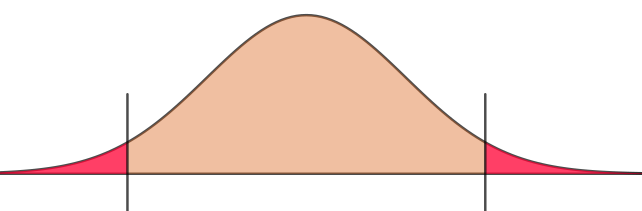
\includegraphics[width=6cm]{Images/acceptance_region}};
	\draw [color=black](-0.7,.3) node[anchor=north west] {$1-\alpha$};
	\draw [color=black](0.6,1.) node[anchor=north west] {$f_T\big|_{H_0}$};
	\draw [color=red!40!black](-2.95,-0.6) node[anchor=north west] {$W_L$};
	\draw [color=red!40!black](1.7,-0.6) node[anchor=north west] {$W_U$};
	\draw [color=red!40!black](-2.8,0.2) node[anchor=north west] {$\frac{\alpha}{2}$};
	\draw [color=red!40!black](1.7,0.2) node[anchor=north west] {$\frac{\alpha}{2}$};
	\draw [color=red!40!black](3.0,0.2) node[anchor=north west] {$W_\alpha=W_L\cup W_U$};
	\draw [color=black](-1.8,-0.7) node[anchor=north west] {Acceptance region};
	\draw [color=black](-0.7,-1.1) node[anchor=north west] {$A(\t_0)$};
	\end{tikzpicture}
	\caption{Souvislost $\mathrm{CI}_{1-\alpha}$ a~testování hypotézy $H_0:\t=\t_0$ skrze CR $W_\alpha$.}
	\label{obrazek}
\end{figure}
\end{remark}

Mějme  nyní náš statistický model $\PP\in\mathscr{P}$, parametr zájmu $\t=\t(\PP)$ a~náhodný výběr $X_1,...,X_n~iid~\PP_{\t}$.
\subsection*{Metoda konstrukce $\mathrm{CM}_{1-\alpha}$ pro~$\t$:}
\begin{enumerate}[1.]
	\item Volíme $\t_0\in\Theta$ libovolně pevně.
	\item Testujeme $H_0:\t=\t_0$ na~hladině významnosti $\alpha$. Příslušný test označíme $\crossedphi_\alpha$, resp. $W_\alpha$ pro~případ neznáhodněného testu.
	\item Vyjádříme $A(\t_0)$ pro~test $\crossedphi_\alpha$, resp. $W_\alpha$, při~libovolném $\t_0\in\Theta$. Tím získáme $A(\t)$ pro~$\forall\t\in\Theta$.
	\item Pak $C(\X)=\left\{ \t\in\Theta:\X\in A(\t) \right\}$ je $\mathrm{CM}_{1-\alpha}$ pro~$\t$. Navíc, pokud je test $\crossedphi_\alpha$ neznáhodněný a~je na~hladině $\alpha$, $\beta_{\crossedphi_\alpha}(\t_0)=\alpha$ pro~$\forall\t_0\in\Theta$, pak uvedená $C(\X)$ je $\mathrm{CM}_{1-\alpha}$ s~\textbf{konfidenčním koeficientem} rovným $(1-\alpha)$.
	\begin{proof}
		Ukážeme tvrzení z~bodu 4 pro~případ identifikovatelné rodiny $\mathscr{P}=\{\PP_\t\}$, ve~které je $\t$ jediným parametrem modelu (nejsou zde tzv. rušivé parametry):\[
		\begin{split}
		\inf\limits_{\PP\in\mathscr{P}}\PP\br{\t\in C(\X)}&=\inf\limits_{\t\in\Theta} \PP_{\t}\br{\t\in C(\X)}=\inf\limits_{\t\in\Theta} \PP_\t\br{\X\in A(\t)}=1-\sup\limits_{\t\in\Theta} \PP_\t\br{\X\notin A(\t)}=\\&=1-\underbrace{\sup\limits_{\t\in\Theta} \PP_\t\br{\crossedphi_\alpha(\X,\t)=1}}_{\leq\alpha}\geq 1-\alpha.
		\end{split}
		\]
	\end{proof}
\end{enumerate}
\begin{remark}
	Pokud $C(\X)$ vznikne prostřednictvím \textbf{neznáhodněného} UMP testu $\crossedphi_\alpha$ na~hladině $\alpha$ pro~$\forall\t_0\in\Theta$, pak $C(\X)$ nazveme UMA (\textit{uniformly most accurate}) $\mathrm{CM}_{1-\alpha}$ pro~$\t$. Podobně použitím $\txt{UMPU}$ testu na~hladině $\alpha$ získáme UMAU$_{1-\alpha}$ (\textit{UMA Unbiased, CM$_{1-\alpha}$}) pro~$\t$.
\end{remark}
\begin{example}
	Uvažujme statistický model $X_1,...,X_n~iid~\n{\mu,\sigma^2}$, kde $\sigma^2>0$ je neznámé. Jde nám o~$\mathrm{CI}_{1-\alpha}$ pro~parametr $\t=\mu$ na~hladině $\alpha\in(0,1)$. Testujeme pro~$\forall\mu_0\in\R$ hypotézu
	$$\hypothesiswide{\mu=\mu_0}{\mu\neq\mu_0}\quad\text{ na~hladině }\alpha.$$
	Použijeme LRT$_\alpha$ test s~příslušnou LRT kritickou oblastí
	$$ W_\alpha=\bigg\{ \textbf{x}:\abs{\frac{\sqrt{n}(\oxnn-\mu_0)}{s_n}}\geq \underbrace{t_{1-\frac{\alpha}{2}}(n-1)}_{K_\alpha} \bigg\},\quad\text{pro }\forall\mu_0\in\R. $$ Pak přípustná oblast pro~$\forall\mu_0\in\R$ je rovna 
	$$ A(\mu_0)=W_\alpha^c=\left\{ \textbf{x}:\abs{\frac{\sqrt{n}(\oxnn-\mu_0)}{s_n}}<t_{1-\frac{\alpha}{2}}(n-1) \right\} $$ nezávisle na~neznámém (rušivém) parametru $\sigma^2>0$. Pak podle bodu 4 konstrukce,
	$$ C(\X)=\left\{ \mu\in\R:\X\in A(\mu) \right\}=\abs{\begin{array}{l}
	\text{řešení příslušné}	\\ \text{nerovnosti v~}A(\mu) 
		\end{array} }=\Br{\Oxn-t_{1-\frac{\alpha}{2}}(n-1)\frac{s_n}{\sqrt{n}},\Oxn+t_{1-\frac{\alpha}{2}}(n-1)\frac{s_n}{\sqrt{n}}} $$
	je CI pro~$\mu$ s~konfidenčním koeficientem rovným $1-\alpha$. Tento CI je shodný s~CI$_{1-\alpha}$ získaným v~příkladu \ref{priklad} prostřednictvím pivotální náhodné veličiny $T(\X)$ (t-statistika).
\end{example}
\begin{remark}
	Všimněte si, že v~obou konstrukcích CM$_{1-\alpha}$ pomocí PQ pivotů nebo $\crossedphi_\alpha$ testů jsme neřešili velikost středního objemu/délky tohoto $C(\X)$, tzn. stejnoměrnou minimalizaci $\EE{\lambda\br{C(\X)}}$. Většinou je to úloha obtížná, mnohdy (explicitně) neřešitelná, na~stejné úrovni jako je úloha nalezení testu $\crossedphi_\alpha$ se~stejnoměrně maximální silofunkcí (silou) testu $\beta_{\crossedphi_\alpha}\big|_{H_1}$.
\end{remark}
\section{Asymptotické konfidenční množiny}
\begin{define}
	Mějme $\PP\in\mathscr{P}$ na~$(\Omega,\Aa),~\t=\t(\PP)\in\Theta\subset \R^1$, resp. $\Theta\subset\R^k$ a~$\Bb_\Theta$ Borelovské. Mějme $X_1,...,X_n\sim\PP\in\mathscr{P}$ a~$\alpha\in(0,1)$. Pak $C(\X)\in\Bb_\Theta$ se~nazývá \textbf{asymptotická} CM$_{1-\alpha}$, ozn ACM$_{1-\alpha}$, pokud pro
	$$\forall\PP\in\mathscr{P},\quad \lim\limits_{n\to+\infty}\PP\br{\t\in C(\X)}\geq 1-\alpha.$$
\end{define}
\subsection*{Metody konstrukce:}
\begin{enumerate}[I)]
	\item Najdeme takovou vhodnou náhodnou veličinu $\mathcal{R}_n(\X,\t)$, která je \textbf{asymptoticky pivotální} veličinou (ozn. APQ), tzn. její \textit{limitní} rozdělení nezávisí na~$\PP\in\mathscr{P}$: 
	$$\mathcal{R}_n(\X,\t)\Dto G,\quad\text{kde }G\text{ nezávisí na~}\PP\in\mathscr{P}.$$ 
	Toto limitní $G$ použijeme pro~konstrukci ACM$_{1-\alpha}$ stejně jako v~případě neasymptotických CM$_{1-\alpha}$ (viz sekce \ref{pivoty}).
	\item Stejně jako v~sekci \ref{TSHkonst}, pro~konstrukci ACM$_{1-\alpha}$ použijeme přípustnou oblast $A(\t_0)$ založenou na~asymptotickém testu $\crossedphi_\alpha$ dosahujícím asymptotické hladiny $\alpha$ pro~testování $H_0:\t=\t_0$. Tedy $C(\X)=\left\{ \t\in\Theta:\X\in A(\t)\right\}$, kde $A(\t)$ je AR asymptotického testu $\crossedphi_\alpha$, je ACM$_{1-\alpha}$ pro~parametr $\t$.  
\end{enumerate}
\begin{example}[I]
	Mějme $X\sim\FF\in\mathcal{F}$ a~volme $\t=\t(\FF)=\FF(t)$ pro~nějaké fixní $t\in\R$. Najdeme ACI$_{1-\alpha}$ pro~$\FF(t)$ založený na~$X_1,...,X_n~iid~\FF$ náhodného výběru. Víme, že $$\FF_n(t)=\frac{1}{n}\sumjn \Identita{(-\infty,t]}(X_j)\quad\text{(empirická c.d.f.)}$$ je náhodnou veličinou, která je $\AN$ odhadem $\FF(t)$ pro~$\forall t\in\R$, konkrétně\\ $\FF_n(t)\sim\AN\Br{\FF(t),\frac{1}{n}\FF(t)\br{1-\FF(t)}}$. Pak 
	$$ \mathcal{R}_n(\X)=\frac{\sqrt{n}\br{\FF_n(t)-\FF(t)}}{\sqrt{\FF(t)\br{1-\FF(t)}}}\Dto U\sim\n{0,1}, $$ a~proto $\mathcal{R}_n(\X)$ je APQ veličinou. Volíme $c_2=-c_1=u_{1-\frac{\alpha}{2}}$ kvantil $\n{0,1}$, pro který platí, že
	$$ \lim\limits_{n\to+\infty}\PP_\FF\br{\abs{\mathcal{R}_n(\X)}\leq u_{1-\frac{\alpha}{2}}}= \PP_{\n{0,1}}\br{\abs{U}\leq u_{1-\frac{\alpha}{2}}}=1-\alpha. $$
			Vyřešením nerovnosti $\abs{\mathcal{R}_n(\X)}\leq u_{1-\frac{\alpha}{2}}$ vzhledem k~$\FF(t)$ pak snadno dostaneme ACI$_{1-\alpha}$ pro~$\FF(t)$ při~fixním $t\in\R$.
\end{example}
\begin{example}[II]
	Mějme opět systém distribucí $\mathscr{P}$, $\t=\t(\PP)\in\Theta\subset\R^k$ a~$X_1,...,X_n~iid~\PP\in\mathscr{P}$. Pro~konstrukci ACM$_{1-\alpha}$ využijeme \textbf{asymptotický LRT} test $\hypothesis{\t=\t_0}{\t\neq\t_0}$ na~hladině $\alpha$ pro $\forall\t_0\in\Theta$. Víme, že za~platnosti $H_0$ a~předpokladu věty 5. má veličina $\lambda_n(\X)=-2\ln\Lambda(\textbf{x})$ asymptotické rozdělení $\chi^2(k)$, tzn. 
	$$ \lambda_n(\X)=-2\ln\frac{L(\t_0)}{L(\htn)}=2\br{l(\htn)-l(\t_0)}\Dto \chi^2(k)\quad \text{pro~}\forall\t_0\in\Theta, $$  kde $\htn$ je MLE odhad parametru $\t$. Příslušná LRT kritická oblast $W_\alpha=\left\{ \textbf{x}:\Lambda(\textbf{x})\leq K_\alpha \right\}$ vede na přípustnou oblast
	$$A(\t_0)=\left\{ \textbf{x}:\lambda_n(\textbf{x})<-2\ln K_\alpha\equal{\text{ozn}}K_\alpha' \right\}\quad \text{pro~}\forall\t_0,$$ pro~kterou však platí limitní vztah
	$$ \lim\limits_{n\to+\infty} \PP_{\t_0}\br{\X\in A(\t_0)}=\lim\limits_{n\to+\infty} \PP_{\t_0}\big( \underbrace{\lambda_n(\X)}_{\Dto\chi^2(k)}<\chi^2_{1-\alpha}(k) \big)=1-\alpha, $$
	kde jsme použili volbu $K_\alpha'=\chi^2_{1-\alpha}(k)$ kvantil $\chi^2(k)$ rozdělení. Máme tedy ACM$_{1-\alpha}$ pro~parametr $\t$ ve~tvaru 
	$$ C(\X)=\left\{ \t\in\Theta:\X\in A(\t) \right\}=\left\{ \t\in\Theta: l(\htn)<\frac{\chi^2_{1-\alpha}(k)}{2}+l(\t) \right\}. $$
	
\end{example}
\begin{remark}
	ACM$_{1-\alpha}$ $C(\X)$ získaná prostřednictvím asymptotického LRT testu může být podstatně odlišná od~ACM$_{1-\alpha}$ získaná metodou APQ nebo PQ, viz např. \textbf{simultální} ACM$_{1-\alpha}$ oproti CM$_{1-\alpha}$ pro~parametr $\t=(\mu,\sigma^2)$ v~Gaussovském modelu $\n{\mu,\sigma^2}$.
\end{remark}